%!TEX program = xelatex


% 打印选项: 双面打印 twoside;单面打印 oneside
% 模板选项: 硕士论文 master; 博士论文 doctor
% openright, openany 指定新的一章 \chapter 是在奇数页(右侧)开始,还是直接紧跟着上一页开始。report 默认为 openany,book 默认为 openright。对 article 无效。
\documentclass[twoside, doctor, openany]{ecust_thesis}
\usepackage{amssymb,amsfonts,amsmath,mathrsfs}
\allowdisplaybreaks[4] % 长公式换页
\usepackage{bm} % 加粗数学公式

\AtBeginDocument{% 修改公式上下间距 https://tex.stackexchange.com/questions/69662/how-to-globally-change-the-spacing-around-equations
 \abovedisplayskip=5pt plus 4pt minus 2pt
 \abovedisplayshortskip=5pt plus 4pt minus 4pt
 \belowdisplayskip=5pt plus 4pt minus 2pt
 \belowdisplayshortskip=5pt plus 4pt minus 4pt
}

\usepackage{enumerate}
\usepackage{multirow}
\usepackage{algpseudocode} % 算法包
\usepackage{algorithmicx} % 算法包
\usepackage[chapter]{algorithm} % 算法按章编号
% \renewcommand{\thealgorithm}{\arabic{chapter}.\arabic{algorithm}}
%\usepackage{arydshln} % 在引用longtable包的情况下,arydshln包会和booktab包冲突
\usepackage[list=off]{bicaption}% ccaption -- bicaption
\usepackage{longtable}
\setlength{\LTpre}{0pt} % 设置longtable的前后间距 https://tex.stackexchange.com/questions/5683/how-to-remove-top-and-bottom-whitespace-of-longtable
\setlength{\LTpost}{0pt}
\usepackage{threeparttable}
\usepackage{tabularx}
\makeatletter
\newcommand{\multiline}[1]{% 表格中的多行
  \begin{tabularx}{\dimexpr\linewidth-\ALG@thistlm}[t]{@{}X@{}}
    #1
  \end{tabularx}
}
\newcommand{\tabincell}[2]{\begin{tabular}{@{}#1@{}}#2\end{tabular}}
\makeatother
\usepackage[figuresright]{rotating} % 用于旋转表:
\usepackage{float} % 设置表格位置 \begin{table}[H] % 用H表示必须放在这里
% \restylefloat{table} % https://stackoverflow.com/questions/1673942/latex-table-positioning
\usepackage{balance}
\usepackage{autobreak}
\usepackage{graphicx}
\usepackage{epsfig}
\usepackage{color}
\usepackage[normalem]{ulem} % underline
\usepackage{CJKulem} % 使用Ctex,ulem宏包中下划线命令\uline如果对中文处理,则中文换行失效,需要换成一下Ctex专用宏包。
\usepackage[utf8x]{inputenc}
\usepackage{textcomp}

\usepackage{pdfpages} % 用于合并pdf

% \usepackage[bookmarksopen=true]{hyperref}
\usepackage{bookmark} % 把不编号章节仅加入PDF书签,不放入目录

\usepackage{paralist}
\let\itemize\compactitem
\let\enditemize\endcompactitem
\let\enumerate\compactenum
\let\endenumerate\endcompactenum
\let\description\compactdesc
\let\enddescription\endcompactdesc
\setdefaultleftmargin{2em}{2em}{1em}{1em}{1em}{1em} % 调整itemize对齐

\usepackage{titlesec} % 设置垂直对齐方式,\flushbottom垂直两端对齐(标题不会出现在页尾),\raggedbottom顶部对齐
\raggedbottom

% \renewcommand{\thefootnote}{\fnsymbol{footnote}} % footnote格式https://www.overleaf.com/learn/latex/Footnotes

%% 定义常用的符号
\newcommand{\ssd}{{$^\circ$C}} %℃
\newcommand{\hsd}{{$^\circ$F}} %℉
\newcommand{\blh}{\textasciitilde} % 波浪号~

% \theoremstyle{plain} % 默认,这几个命令改变remark中的字体样式
% \theoremstyle{remark}
\theoremstyle{definition}
\newtheorem{definition}{定义}[chapter]
\newtheorem{remark}{注}[chapter]

%\allowdisplaybreaks % 使大公式跨页显示,以补充前一页底部的空白。
\interdisplaylinepenalty=2500
\hyphenpenalty=5000 % 通过调整单词断开位置调整段落右边对齐效果
\tolerance=1200

\renewcommand{\algorithmicrequire}{\textbf{Input:}}
\renewcommand{\algorithmicensure}{\textbf{Output:}}
%\renewcommand{\algorithmicfor}{\textbf{对}}
%\renewcommand{\algorithmicif}{\textbf{如果}}
%\renewcommand{\algorithmicdo}{\textbf{执行}}
%\renewcommand{\algorithmicelse}{\textbf{否则}}
%\renewcommand{\algorithmicthen}{\textbf{则}}
%\renewcommand{\algorithmicend}{\textbf{结束}}

\begin{document}

%%%%%%%%%%%%%%%%%%%%%%%%%%%%%%
%% 封面
%%%%%%%%%%%%%%%%%%%%%%%%%%%%%%

\title{DelaySSA中文文档}
% \englishtitle{
%   \begin{tabular}{c}
%     两行英文标题 \\ 换行方式
%   \end{tabular}}
% \englishauthor{}

% \includepdf[pages=-]{chapters/硕、博士封面.pdf}
% \includepdf[pages=-]{chapters/空白页.pdf}
% \includepdf[pages=-]{chapters/学位论文扉页.pdf}
% \includepdf[pages=-]{chapters/学位论文授权声明.pdf}
% \includepdf[pages=-]{chapters/空白页.pdf}
% \includepdf[pages=-]{chapters/学位论文提交要求.pdf}
% \includepdf[pages=-]{chapters/空白页.pdf}
% \includepdf[pages=-]{chapters/作者声明.pdf}
% \includepdf[pages=-]{chapters/空白页.pdf}
%% 上面资料下载地址:https://gschool.ecust.edu.cn/12735/list.htm

%%%%%%%%%%%%%%%%%%%%%%%%%%%%%%
%% 前置部分
%%%%%%%%%%%%%%%%%%%%%%%%%%%%%%
\frontmatter

% 摘要

\begin{abstract}
本模板针对有一定LaTeX基础的同学,提供了华东理工大学博士学位论文写作模板,简要给出了图、表、算法等示例。
如果读者对LaTeX还不熟悉,建议以参考文献\cite{LaTeX2e介绍}作为入门。


\keywords{华东理工大学;毕业论文;LaTeX}
\end{abstract}



\begin{englishabstract}
This is English abstract.

\englishkeywords{AAA; BBB; CCC}

\end{englishabstract}



% 加入目录
\tableofcontents
\cleardoublepage % 保证第一章的位置
%% 加入表格索引
%%\listoftables
% 加入插图索引
%\listoffigures


%%%%%%%%%%%%%%%%%%%%%%%%%%%%%%
%% 正主体部分
%%%%%%%%%%%%%%%%%%%%%%%%%%%%%%
\mainmatter

%% 各章正文内容

\chapter{简介}


随机模拟算法(SSA)广泛用于模拟具有马尔可夫动力学的复杂系统的时变轨迹(Gillespie,1977)\upcite{BITthesis}。
这些模型背后的一个主要假设是无记忆假设,即反应物的随机动力学仅受系统当前状态的影响,这意味着连续反应事件之间的等待时间遵循指数分布。


许多常见的反应系统封装了涉及大量相互作用物质的多个中间反应步骤(Filatova等人,2021)\upcite{BITthesis}。
这就导致使用SSA进行随机模拟时需要高昂的计算成本,严重限制了在很大一部分参数空间中对动力学过程的探索。
一种可行的替代方法是使用简化模型。虽然理论上如果存在时间尺度分离,就可以进行严格的分析进行模型简化(Mastny et al.,2007;Kan et al.,2016),
但是在实际情况下,通常用一个延迟反应来代替多个中间反应。
通过这种方法就可以获得一个具有非马尔可夫动力学的简化模型,即连续反应事件之间的等待时间是非指数的,这是传统SSA无法模拟的。


几种具有延迟的反应系统的精确模拟方法已经被提出(Barrio等人,2006;Cai,2007;Anderson,2007;Ramaswamy和Sbalzarini,2011)。
其中一些方法可通过软件工具实现(Maarleveld等人,2013年;Barbuti等人,2009年)。
然而,这些软件包提供的功能有限(只能实现少量延迟SSA算法,并且仅限于固定延迟或质量作用反应),对于潜在的用户群来说,功能非常局限。


我们提供的DelaySSAToolkit.jl是首个用于建模时滞随机反应系统的Julia软件包。
反应中的延迟可以是固定的,也可以是随时间变化的,即每次触发延迟反应时,可以从用户定义的概率分布中选择延迟。
还可以对存在相同反应物系统总体的非均相时滞情况进行建模,其中每个反应物系统都有一个具有不同但固定时滞的反应。
此外,此软件包还可以使用各种延迟随机模拟算法集成同步延迟反应和延迟反应级联。
有关Delay SSA理论和软件使用教程的全面教程,请访问https://github.com/palmtree2013/DelaySSAToolkit.jl。 


\section{模型与方法}

延迟反应系统的定义包括两部分,即反应发生瞬间就影响反应物状态的马尔可夫部分和反应发生在一定时间延迟$\tau$后,反应物状态才发生变化的非马尔可夫部分(图1a)。
反应网络的马尔可夫部分可以通过使用Julia符号数字建模框架————Catalyst.jl(https://github.com/SciML/Catalyst.jl)和ModelingToolkit.jl(Ma等人,2021)工具包,再指定化学计量比和反应倾向来构建。
另一种方法是使用较低级别的编程接口————DifferqJump.jl(https://github.com/SciML/DiffEqJump.jl)工具包,手动定义每个反应的化学计量数和倾向函数。 

DelaySSAToolkit.jl通过指定即时反应和由其触发的延迟反应之间的因果关系,将上述定义的马尔可夫模型扩展到延迟系统。
因此,DelaySSAToolkit.jl可以处理包含任意数量物质和反应的非马尔可夫系统,其中系统中的物质和反应可以是任意类型的光滑倾向函数和广泛的延迟类型。



DelaySSAToolkit.jl的算法实现是基于DiffEqJump.jl提供的SSA算法和DiffEqJump.jl提供的解决算法处理程序。
它目前支持四种延迟随机模拟算法:延迟拒绝法(Bratsun et al.,2005;Barrio et al.,2006)、延迟直接法(Cai,2007)、延迟修正下一反应法(Anderson,2007)
和具有组成和拒绝的延迟直接法(Slepoy et al.,2008;Mauch和Stalzer,2011)。
延迟拒绝法和延迟直接方法在反应数量小的反应网络表现的性能更好,而其他两种方法则更适合于反应数量较多的系统。
使用(Gibson和Bruck,2000)中描述的依赖图和优先级队列,提高了反应数量较多的大规模网络中延迟修正下一反应法和具有组合和拒绝的延迟直接法的计算效率。
使用DifferentialEquations.jl中提供的高性能多线程/多处理并行计算接口,可以轻松实现集成仿真。同时这个工具包还提供了一些数值分析和参数估计工具,可以进一步研究由它产生的延迟系统。
延迟SSA问题的结果可以依据用户指定的需要,造时间点或在确切的事件时间点给出。每个SSA问题的结果的数据结构由三部分组成:时间点、反应物状态和对应时间点的延迟通道状态。
延迟通道的记录状态在某些情况下特别有用,例如,当模拟基因转录时,延迟反应用于模拟转录起始和终止之间的时间,并且从延迟通道的状态可以重建RNA聚合酶在基因上的位置(Fu等人,2021)。 


% 
\chapter{模板说明}\label{c1:intro}

本模板基于\verb|北京理工大学硕士(博士)学位论文LaTeX模板|\upcite{BITthesis}修改。
修改内容主要包括:
\begin{enumerate}
  \item 页眉页脚样式、高度、页边距;
  \item 左右页边距;
  \item 行间距;
  \item 公式、图、表前后间距;
  \item 各级标题前后间距和样式;
  \item 列表、枚举的缩进;
  \item 其他样式等。
\end{enumerate}

下面给出论文中常用的各类图、表、算法、公式、参考文献等的使用方法。

\begin{remark}
  本文默认读者已经知道了LaTeX的基本语法,并可以熟练使用LaTeX写期刊论文。
  下面仅介绍重要的、常用的示例,并不加以详细解释。
\end{remark}

\section{编译}

编译顺序为:xelatex-->bibtex-->xelatex-->xelatex。

推荐使用VSCode + LaTeX Workshop的组合写论文。

\section{图}\label{c1sec:figure}

图\ref{c1fig_demo1}是一个标准的图。
\begin{figure}[!htb]
  \centering
  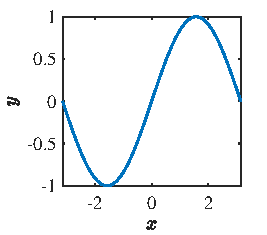
\includegraphics[width=5cm]{figures/chapter1/fig_demo.pdf}
  \bicaption{示意图}
  {Demo}
  \label{c1fig_demo1}
\end{figure}

图\ref{c1fig_demo2}是一行多列的子图安排方式。
\begin{figure}[!htb]
  \centering
  \subfigure[]{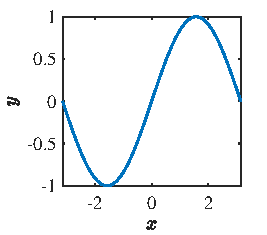
\includegraphics[width=0.28\textwidth]{figures/chapter1/fig_demo.pdf}}
  \subfigure[]{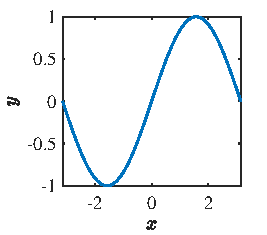
\includegraphics[width=0.28\textwidth]{figures/chapter1/fig_demo.pdf}}
  \bicaption{一行多列的子图安排方式。
  (a) 子图1,
  (b) 子图2}
  {Subfigure. 
  (a) subfigure 1,
  (b) subfigure 2} 
  \label{c1fig_demo2}
\end{figure}

图\ref{c1fig_demo3}是多行多列的子图安排方式。如果想让这段话出现在图\ref{c1fig_demo2}之后,则可以在图\ref{c1fig_demo2}中使用\verb|\begin{figure}[H]|命令。
\begin{figure}[H]
  \centering
  \subfigure[当然,如果你想,这里也可以写些内容]{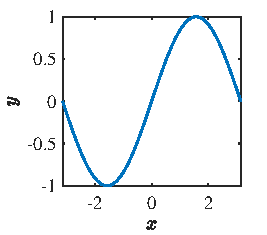
\includegraphics[width=0.28\textwidth]{figures/chapter1/fig_demo.pdf}}
  \subfigure[]{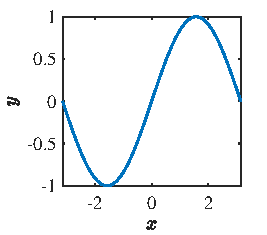
\includegraphics[width=0.28\textwidth]{figures/chapter1/fig_demo.pdf}}\\
  \subfigure[]{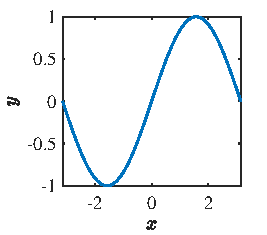
\includegraphics[width=0.28\textwidth]{figures/chapter1/fig_demo.pdf}}
  \subfigure[]{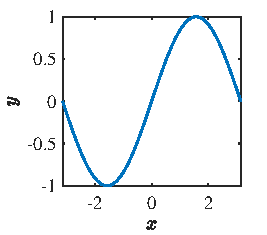
\includegraphics[width=0.28\textwidth]{figures/chapter1/fig_demo.pdf}}
  \bicaption{子图示意图。
  (a) 子图1,
  (b) 子图2,
  (c) 子图3,
  (d) 子图4}
  {Subfigure. 
  (a) subfigure 1,
  (b) subfigure 2,
  (c) subfigure 3,
  (d) subfigure 4} 
  \label{c1fig_demo3}
\end{figure}

% \newpage
\section{表格}\label{c1sec:table}

表\ref{c1tab_1}是一个标准的三线表格。
\begin{table}[H]
  \zihao{5} 
  \renewcommand{\arraystretch}{1.3}
  \renewcommand{\tabcolsep}{5pt}
  \bicaption{这是一个标准表格}
  {This is a standard table}
  \label{c1tab_1}
  \centering
  \begin{tabular}{cc}
  \toprule
  名称1 & 名称2 \\
  \midrule
  A	&	B	\\
  A	&	B	\\
  \bottomrule
  \end{tabular}
\end{table}

表\ref{c1tab_2}是一个带脚注的复杂表格。可以看到这段文字没有出现在上一页的末尾(尽管上一页的末尾还有空间),是因为表\ref{c1tab_1}中使用了\verb|\begin{table}[H]|命令。
\begin{table}[!htb]
  \zihao{5} 
  \renewcommand{\arraystretch}{1.3}
  \renewcommand{\tabcolsep}{5pt}
  \bicaption{这是一个带脚注的复杂表格\textsuperscript{a}}
  {This is a complex table}
  \label{c1tab_2}
  \centering
  \begin{tabular}{ccccccc}
  \toprule
  \multirow{3}{*}{AAA}	&	\multicolumn{2}{c}{BBB\textsuperscript{b}}	&	\multicolumn{2}{c}{CCC}	&	\multicolumn{2}{c}{DDD}	\\
  \cmidrule(r){2-3} \cmidrule(r){4-5} \cmidrule(r){6-7}
    &	\tabincell{c}{A1\\A2}	&	\tabincell{c}{B1\\B2}	&	\tabincell{c}{C1\\C2}	&	\tabincell{c}{D1\\D2}	&	\tabincell{c}{E1\\E2}	&	\tabincell{c}{F1\\F2}	\\
  \midrule
  AAA1	&	20361	&	27.02	&	20901	&	27.72	&	21711	&	28.14	\\
  AAA2	&	10051	&	13.34	&	10051	&	13.33	&	10311	&	13.36	\\
  \bottomrule
  \end{tabular}\\
  \textsuperscript{a} 脚注1 \\
  \textsuperscript{b} 脚注2 \\
\end{table}

表\ref{c1tab_3}是一个较宽的表格,需要缩放到页宽范围,这可以通过命令\\
\verb|\resizebox{1\textwidth}{!}{}|\\
实现。
此表格还采用了\verb|\specialrule{0pt}{3pt}{3pt}|命令来调整倒数第3行-倒数第2行的间距,使表格更美观。

\begin{table}[H]
  \zihao{5} 
  \bicaption{这是一个较宽的表格,需要缩放到页宽范围}
  {This is a complex table}
  \label{c1tab_3}
  \centering
  \resizebox{1\textwidth}{!}{ % 通过缩放,让宽表和正文一样宽
  \begin{tabular}{ccccccc}
  \toprule
  AAA	&	$\delta$	&	$\beta$\textsuperscript{\emph{a}}	&	\tabincell{c}{XXXXXXXXXXXX\\YYY}	&	\tabincell{c}{XXXXXXXXXXXX\\YYY}	&	\tabincell{c}{XXXXXXXXXXXX\\YYY}	&	\tabincell{c}{XXXXXXXXXXXX\\YYY}	\\
  \midrule
  \multirow{4}{*}{AAA}	&	2.549	&	2.549	&	30/30	&	30/30	&	30/30	&	30/30	\\
    &	AAA	&	2.718	&	30/30	&	30/30	&	30/30	&	30/30	\\
    &	AAA	&	3.094	&	30/30	&	30/30	&	30/30	&	30/30	\\
    &	AAA	&	3.200	&	30/30	&	30/30	&	30/30	&	30/30	\\ \specialrule{0pt}{3pt}{3pt}
  \multirow{2}{*}{BBB}	&	2.128	&	2.128	&	30/30	&	30/30	&	30/30	&	30/30	\\
    &	BBB	&	2.500	&	30/30	&	30/30	&	30/30	&	30/30	\\ 
  \bottomrule
  \end{tabular}}\\
  \textsuperscript{\emph{a}} 脚注1
\end{table}

当然,也可以将表\ref{c1tab_3}缩放到指定宽度,如80\%页面宽度,见表\ref{c1tab_4}。

\begin{table}[H]
  \zihao{5} 
  \bicaption{这是一个较宽的表格,需要缩放到80\%页宽范围}
  {This is a complex table}
  \label{c1tab_4}
  \centering
  \resizebox{0.8\textwidth}{!}{ % 通过缩放,让宽表和正文一样宽
  \begin{tabular}{ccccccc}
  \toprule
  AAA	&	$\delta$	&	$\beta$\textsuperscript{\emph{a}}	&	\tabincell{c}{XXXXXXXXXXXX\\YYY}	&	\tabincell{c}{XXXXXXXXXXXX\\YYY}	&	\tabincell{c}{XXXXXXXXXXXX\\YYY}	&	\tabincell{c}{XXXXXXXXXXXX\\YYY}	\\
  \midrule
  \multirow{4}{*}{AAA}	&	2.549	&	2.549	&	30/30	&	30/30	&	30/30	&	30/30	\\
    &	AAA	&	2.718	&	30/30	&	30/30	&	30/30	&	30/30	\\
    &	AAA	&	3.094	&	30/30	&	30/30	&	30/30	&	30/30	\\
    &	AAA	&	3.200	&	30/30	&	30/30	&	30/30	&	30/30	\\ \specialrule{0pt}{3pt}{3pt}
  \multirow{2}{*}{BBB}	&	2.128	&	2.128	&	30/30	&	30/30	&	30/30	&	30/30	\\
    &	BBB	&	2.500	&	30/30	&	30/30	&	30/30	&	30/30	\\ 
  \bottomrule
  \end{tabular}}\\
  \textsuperscript{\emph{a}} 脚注1
\end{table}


如果表格缩放到页面宽度后字体太小看不清,这时你可能需要通过使用\\
\verb|\begin{sidewaystable}|命令来实现一个横着放置的宽表,如表\ref{c1tab_5}所示。

\begin{sidewaystable}
  \zihao{5} 
  \renewcommand{\arraystretch}{1.2}
  % \renewcommand{\tabcolsep}{3pt}
  \bicaption{sidewaystable表格}
  {sidewaystable}
  \label{c1tab_5}
  \centering
  \begin{tabular}{ccc|cc|cc}
  \toprule
  Problem	&	AAA1	&	AAA2	&	BBB1	&	BBB2	&	CCC1	&	CCC2	\\
  \midrule
  ABC1	&	5.51e-01(8.20e-02)	&	\textbf{8.23e-01(1.75e-02)+ }	&	3.17e-02(3.99e-02)	&	\textbf{8.46e-01(9.72e-03)+ }	&	8.32e-01(9.47e-03)	&	\textbf{8.71e-01(1.51e-04)+ }	\\
  ABC2	&	2.38e-01(7.85e-02)	&	\textbf{4.81e-01(2.22e-02)+ }	&	0.00e+00(0.00e+00)	&	\textbf{9.77e-02(1.99e-01)+ }	&	4.48e-01(7.58e-02)	&	\textbf{5.38e-01(1.63e-04)+ }	\\
  ABC3	&	4.83e-01(6.85e-02)	&	\textbf{8.83e-01(9.03e-02)+ }	&	9.19e-02(6.93e-02)	&	\textbf{9.82e-01(3.03e-02)+ }	&	9.71e-01(1.49e-02)	&	\textbf{1.02e+00(3.01e-04)+ }	\\
  ABC4	&	0.00e+00(0.00e+00)	&	\textbf{5.83e-01(1.33e-01)+ }	&	0.00e+00(0.00e+00)	&	\textbf{9.58e-02(2.51e-01)+ }	&	1.55e-01(1.53e-01)	&	\textbf{6.77e-01(1.16e-01)+ }	\\
  ABC6	&	3.73e-01(7.27e-02)	&	\textbf{4.10e-01(2.62e-02)= }	&	1.39e-01(1.63e-01)	&	\textbf{1.79e-01(1.76e-01)= }	&	1.20e-01(7.40e-02)	&	\textbf{4.33e-01(1.39e-04)+ }	\\
  ABD1	&	1.21e+01(1.64e+00)	&	\textbf{4.31e+01(2.54e+00)+ }	&	1.58e+01(8.86e-01)	&	\textbf{4.49e+01(2.04e+00)+ }	&	2.74e+01(2.15e+00)	&	\textbf{3.34e+01(3.46e+00)+ }	\\
  ABD2	&	\textbf{5.54e+01(7.97e-01)}	&	5.51e+01(1.11e+00)= 	&	5.66e+01(5.68e-01)	&	\textbf{5.87e+01(3.75e-01)+ }	&	5.81e+01(4.11e-01)	&	\textbf{5.86e+01(3.19e-01)+ }	\\
  ABD4	&	2.86e+01(6.99e-01)	&	\textbf{3.27e+01(3.69e-01)+ }	&	3.06e+01(4.13e-01)	&	\textbf{3.40e+01(2.81e-01)+ }	&	3.38e+01(2.36e-01)	&	\textbf{3.49e+01(1.85e-01)+ }	\\
  ABD5	&	2.95e+01(3.10e-01)	&	\textbf{2.98e+01(4.45e-01)+ }	&	3.06e+01(2.38e-01)	&	\textbf{3.09e+01(2.48e-01)+ }	&	3.23e+01(2.38e-01)	&	\textbf{3.29e+01(1.74e-01)+ }	\\
  ABD6	&	2.47e+01(1.83e+00)	&	\textbf{2.83e+01(1.82e+00)+ }	&	2.67e+01(1.28e+00)	&	\textbf{2.98e+01(1.03e+00)+ }	&	3.08e+01(8.79e-01)	&	\textbf{3.12e+01(5.63e-01)= }	\\
  ABD7	&	2.87e+01(1.44e+00)	&	\textbf{3.25e+01(3.74e-01)+ }	&	3.22e+01(5.55e-01)	&	\textbf{3.41e+01(2.05e-01)+ }	&	3.40e+01(2.16e-01)	&	\textbf{3.44e+01(2.60e-01)+ }	\\
  ABD8	&	1.93e+01(2.52e+00)	&	\textbf{2.60e+01(8.95e-01)+ }	&	2.50e+01(6.55e-01)	&	\textbf{2.76e+01(2.78e-01)+ }	&	2.82e+01(3.08e-01)	&	\textbf{2.83e+01(3.76e-01)= }	\\
  ABD9	&	2.85e+01(1.72e+00)	&	\textbf{2.97e+01(1.87e+00)+ }	&	3.07e+01(1.21e+00)	&	\textbf{3.14e+01(1.74e+00)+ }	&	3.19e+01(7.18e-01)	&	\textbf{3.26e+01(3.73e-01)+ }	\\
  ABE1	&	4.93e-03(1.36e-02)	&	\textbf{1.09e-01(3.94e-02)+ }	&	2.70e-02(4.19e-02)	&	\textbf{1.09e-01(4.31e-02)+ }	&	5.89e-02(5.15e-02)	&	\textbf{8.66e-02(5.55e-02)+ }	\\
  ABE2	&	6.23e-01(2.53e-02)	&	\textbf{7.06e-01(1.98e-03)+ }	&	7.14e-01(2.33e-03)	&	\textbf{7.21e-01(2.34e-03)+ }	&	7.39e-01(8.54e-04)	&	\textbf{7.42e-01(4.94e-04)+ }	\\
  ABE3	&	0.00e+00(0.00e+00)	&	0.00e+00(0.00e+00)= 	&	\textbf{1.02e-03(5.60e-03)}	&	0.00e+00(0.00e+00)= 	&	0.00e+00(0.00e+00)	&	\textbf{1.18e-02(6.46e-02)= }	\\
  ABE4	&	5.26e-01(1.33e-01)	&	\textbf{5.34e-01(1.69e-01)= }	&	\textbf{4.76e-01(1.95e-01)}	&	4.57e-01(2.20e-01)= 	&	6.23e-01(1.66e-01)	&	\textbf{6.34e-01(1.42e-01)= }	\\
  ABE5	&	1.28e-01(6.25e-04)	&	\textbf{1.30e-01(1.27e-04)+ }	&	\textbf{1.26e-01(7.35e-04)}	&	1.25e-01(1.26e-03)- 	&	\textbf{1.29e-01(6.99e-04)}	&	1.28e-01(1.81e-03)= 	\\
  ABE6	&	1.09e-01(4.66e-02)	&	\textbf{1.29e-01(1.86e-03)+ }	&	1.17e-01(2.19e-02)	&	\textbf{1.18e-01(1.11e-02)+ }	&	\textbf{1.27e-01(1.04e-03)}	&	1.23e-01(1.14e-03)- 	\\
  ABE7	&	3.94e-01(2.29e-01)	&	\textbf{1.38e+00(3.38e-02)+ }	&	9.96e-02(1.76e-01)	&	\textbf{1.57e+00(3.60e-02)+ }	&	1.43e+00(5.21e-02)	&	\textbf{1.57e+00(1.15e-02)+ }	\\
  \midrule
  +/-/=	&		&	16/0/4	&		&	16/1/3	&		&	14/1/5	\\
  \bottomrule
  \end{tabular}
\end{sidewaystable}

\clearpage
如果一个表太长,则可能需要跨页表格,如表\ref{c1tab_long}所示。
\begin{center}
  \zihao{5} % 图、表、算法
  %\renewcommand{\arraystretch}{1.3} % longtable中的间距默认和正文一样
  \begin{longtable}{llrrr}
  \bicaption{这是一个长表}{This is a very long table}
  \label{c1tab_long} \\
  \toprule
  Name1	&	Name2	&	Name3	&	Name4	&	Name5	\\
  \midrule
  \endfirsthead
  \multicolumn{5}{r}{(接上表)}   \\
  \toprule
  Name1	&	Name2	&	Name3	&	Name4	&	Name5	\\
  \midrule
  \endhead
  AAA	&	A1	&	180.0	&	281.0	&	235.3	\\
      &	A2	&	5.3	&	43.5	&	35.1	\\
      &	A3	&	680.3	&	1020.0	&	759.3	\\
      &	A4	&	14.4	&	15.8	&	15.4	\\
      &	A5 	&	347.7	&	365.0	&	355.9	\\
      &	A6 	&	363.4	&	384.1	&	372.6	\\
      &	A7 	&	373.5	&	393.7	&	384.2	\\
      &	A8 	&	384.9	&	400.0	&	394.4	\\
      &	A9 	&	379.9	&	400.0	&	390.2	\\
      &	A10	&	379.5	&	399.7	&	390.2	\\
      &	A11	&	382.1	&	399.9	&	393.2	\\
  BBB	&	B1	&	895.8	&	918.8	&	907.2	\\
      &	B2	&	0.5	&	1.1	&	0.9	\\
      &	B3	&	715.6	&	2655.0	&	1360.1	\\
      &	B4	&	318.2	&	424.8	&	378.2	\\
      &	B5	&	183.0	&	242.0	&	215.0	\\
      &	B6	&	291.0	&	376.0	&	331.8	\\
      &	B7	&	373.0	&	452.0	&	429.6	\\
      &	B8	&	469.0	&	520.0	&	501.1	\\
      &	B9	&	521.0	&	565.0	&	549.5	\\
  CCC	&	C1&	912.7	&	947.5	&	929.2	\\
      &	C2	&	0.2	&	0.8	&	0.3	\\
      &	C3	&	143.0	&	229.0	&	184.7	\\
      &	C4	&	202.0	&	263.0	&	221.6	\\
      &	C5	&	243.0	&	304.0	&	269.9	\\
      &	C6	&	281.0	&	365.0	&	329.9	\\
      &	C7	&	293.0	&	379.0	&	342.3	\\
  DDD	&	D1	&	369.0	&	397.7	&	382.9	\\
      &	D2	&	384.6	&	406.7	&	394.6	\\
      &	D3	&	385.1	&	407.8	&	397.6	\\
      &	D4	&	388.3	&	405.1	&	398.7	\\
      &	D5	&	385.6	&	407.9	&	397.2	\\
      &	D6	&	387.4	&	414.5	&	401.6	\\
      &	D7	&	388.9	&	418.1	&	403.3	\\
      &	D8 	&	3.6	&	7.2	&	5.3	\\
      &	D9 	&	2.3	&	5.2	&	3.6	\\
      &	D10	&	11.8	&	23.9	&	17.6	\\
      &	D11	&	9.7	&	21.3	&	14.6	\\
      &	D12	&	34.4	&	42.6	&	39.2	\\
      &	D13	&	7.8	&	32.5	&	19.6	\\
  \bottomrule
  \end{longtable}
\end{center}%



\section{算法}\label{c1sec:algorithm}

下面是一个算法示例。

\begin{algorithm*}[!ht]
  \zihao{5} % 图、表、算法
\bicaption{算法示例}
{Algorithm demo}	
\label{c1alg_demo}
\begin{algorithmic}[1]
\Require{
$p_1$:参数1
\Statex	$p_1$:参数2
\Statex	$p_1$:参数3}
\Ensure{
$o_1$:输出1
\Statex	$o_2$:输出2}
\State    第一条命令   \Comment{第一条命令的注释}        
\While	{$True$}	
  \State /***** 下面代码块的注释 *****/
  \State 相关命令 \Comment{注释}
  \If  {$a=b$} \Comment{If的注释}
      \State 执行相关命令 \Comment{注释}
  \EndIf
  \If  {$c=d$}  
      \State 命令   \Comment{注释}
  \Else	
      \State  命令   \Comment{注释}
  \EndIf
\EndWhile
\Repeat
    \State   $j=j+1$ \Comment{注释}
\Until   {$j >  10$}
\For    {$i=1$ \textbf{to} $10$}
      \State $i=i+1$
\EndFor
\State \Return $o_1$, $o_2$
\end{algorithmic}
\end{algorithm*}


\section{公式}\label{c1sec:equation}

略。
更多公式排版见参考文献\cite{latexlive}。


\section{参考文献}\label{c1sec:reference}

参考文献样式分别上标(如参考文献\upcite{BITthesis,latexlive})和非上标(如参考文献\cite{BITthesis,latexlive},参考文献\cite{BITthesis}和\cite{latexlive})等样式。


\section{其他}\label{c1sec:other}

更多信息请参考文献\cite{BITthesis}。

关于LaTeX的更多知识参考文献\cite{LaTeX2e介绍}。
% 
\chapter{模板说明}\label{c1:intro}

本模板基于\verb|北京理工大学硕士(博士)学位论文LaTeX模板|\upcite{BITthesis}修改。
修改内容主要包括:
\begin{enumerate}
  \item 页眉页脚样式、高度、页边距;
  \item 左右页边距;
  \item 行间距;
  \item 公式、图、表前后间距;
  \item 各级标题前后间距和样式;
  \item 列表、枚举的缩进;
  \item 其他样式等。
\end{enumerate}

下面给出论文中常用的各类图、表、算法、公式、参考文献等的使用方法。

\begin{remark}
  本文默认读者已经知道了LaTeX的基本语法,并可以熟练使用LaTeX写期刊论文。
  下面仅介绍重要的、常用的示例,并不加以详细解释。
\end{remark}

\section{编译}

编译顺序为:xelatex-->bibtex-->xelatex-->xelatex。

推荐使用VSCode + LaTeX Workshop的组合写论文。

\section{图}\label{c1sec:figure}

图\ref{c1fig_demo1}是一个标准的图。
\begin{figure}[!htb]
  \centering
  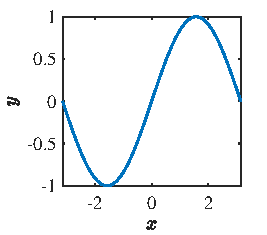
\includegraphics[width=5cm]{figures/chapter1/fig_demo.pdf}
  \bicaption{示意图}
  {Demo}
  \label{c1fig_demo1}
\end{figure}

图\ref{c1fig_demo2}是一行多列的子图安排方式。
\begin{figure}[!htb]
  \centering
  \subfigure[]{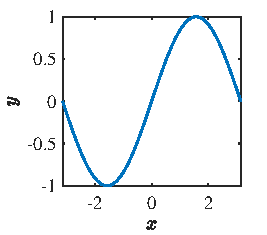
\includegraphics[width=0.28\textwidth]{figures/chapter1/fig_demo.pdf}}
  \subfigure[]{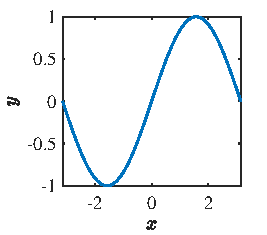
\includegraphics[width=0.28\textwidth]{figures/chapter1/fig_demo.pdf}}
  \bicaption{一行多列的子图安排方式。
  (a) 子图1,
  (b) 子图2}
  {Subfigure. 
  (a) subfigure 1,
  (b) subfigure 2} 
  \label{c1fig_demo2}
\end{figure}

图\ref{c1fig_demo3}是多行多列的子图安排方式。如果想让这段话出现在图\ref{c1fig_demo2}之后,则可以在图\ref{c1fig_demo2}中使用\verb|\begin{figure}[H]|命令。
\begin{figure}[H]
  \centering
  \subfigure[当然,如果你想,这里也可以写些内容]{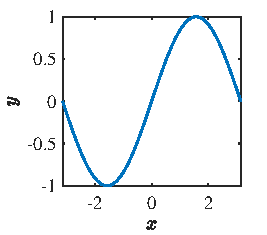
\includegraphics[width=0.28\textwidth]{figures/chapter1/fig_demo.pdf}}
  \subfigure[]{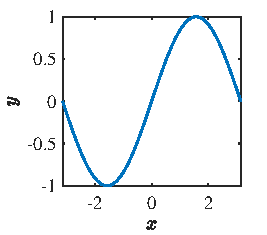
\includegraphics[width=0.28\textwidth]{figures/chapter1/fig_demo.pdf}}\\
  \subfigure[]{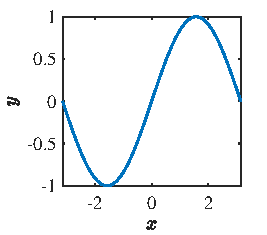
\includegraphics[width=0.28\textwidth]{figures/chapter1/fig_demo.pdf}}
  \subfigure[]{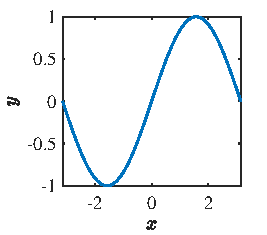
\includegraphics[width=0.28\textwidth]{figures/chapter1/fig_demo.pdf}}
  \bicaption{子图示意图。
  (a) 子图1,
  (b) 子图2,
  (c) 子图3,
  (d) 子图4}
  {Subfigure. 
  (a) subfigure 1,
  (b) subfigure 2,
  (c) subfigure 3,
  (d) subfigure 4} 
  \label{c1fig_demo3}
\end{figure}

% \newpage
\section{表格}\label{c1sec:table}

表\ref{c1tab_1}是一个标准的三线表格。
\begin{table}[H]
  \zihao{5} 
  \renewcommand{\arraystretch}{1.3}
  \renewcommand{\tabcolsep}{5pt}
  \bicaption{这是一个标准表格}
  {This is a standard table}
  \label{c1tab_1}
  \centering
  \begin{tabular}{cc}
  \toprule
  名称1 & 名称2 \\
  \midrule
  A	&	B	\\
  A	&	B	\\
  \bottomrule
  \end{tabular}
\end{table}

表\ref{c1tab_2}是一个带脚注的复杂表格。可以看到这段文字没有出现在上一页的末尾(尽管上一页的末尾还有空间),是因为表\ref{c1tab_1}中使用了\verb|\begin{table}[H]|命令。
\begin{table}[!htb]
  \zihao{5} 
  \renewcommand{\arraystretch}{1.3}
  \renewcommand{\tabcolsep}{5pt}
  \bicaption{这是一个带脚注的复杂表格\textsuperscript{a}}
  {This is a complex table}
  \label{c1tab_2}
  \centering
  \begin{tabular}{ccccccc}
  \toprule
  \multirow{3}{*}{AAA}	&	\multicolumn{2}{c}{BBB\textsuperscript{b}}	&	\multicolumn{2}{c}{CCC}	&	\multicolumn{2}{c}{DDD}	\\
  \cmidrule(r){2-3} \cmidrule(r){4-5} \cmidrule(r){6-7}
    &	\tabincell{c}{A1\\A2}	&	\tabincell{c}{B1\\B2}	&	\tabincell{c}{C1\\C2}	&	\tabincell{c}{D1\\D2}	&	\tabincell{c}{E1\\E2}	&	\tabincell{c}{F1\\F2}	\\
  \midrule
  AAA1	&	20361	&	27.02	&	20901	&	27.72	&	21711	&	28.14	\\
  AAA2	&	10051	&	13.34	&	10051	&	13.33	&	10311	&	13.36	\\
  \bottomrule
  \end{tabular}\\
  \textsuperscript{a} 脚注1 \\
  \textsuperscript{b} 脚注2 \\
\end{table}

表\ref{c1tab_3}是一个较宽的表格,需要缩放到页宽范围,这可以通过命令\\
\verb|\resizebox{1\textwidth}{!}{}|\\
实现。
此表格还采用了\verb|\specialrule{0pt}{3pt}{3pt}|命令来调整倒数第3行-倒数第2行的间距,使表格更美观。

\begin{table}[H]
  \zihao{5} 
  \bicaption{这是一个较宽的表格,需要缩放到页宽范围}
  {This is a complex table}
  \label{c1tab_3}
  \centering
  \resizebox{1\textwidth}{!}{ % 通过缩放,让宽表和正文一样宽
  \begin{tabular}{ccccccc}
  \toprule
  AAA	&	$\delta$	&	$\beta$\textsuperscript{\emph{a}}	&	\tabincell{c}{XXXXXXXXXXXX\\YYY}	&	\tabincell{c}{XXXXXXXXXXXX\\YYY}	&	\tabincell{c}{XXXXXXXXXXXX\\YYY}	&	\tabincell{c}{XXXXXXXXXXXX\\YYY}	\\
  \midrule
  \multirow{4}{*}{AAA}	&	2.549	&	2.549	&	30/30	&	30/30	&	30/30	&	30/30	\\
    &	AAA	&	2.718	&	30/30	&	30/30	&	30/30	&	30/30	\\
    &	AAA	&	3.094	&	30/30	&	30/30	&	30/30	&	30/30	\\
    &	AAA	&	3.200	&	30/30	&	30/30	&	30/30	&	30/30	\\ \specialrule{0pt}{3pt}{3pt}
  \multirow{2}{*}{BBB}	&	2.128	&	2.128	&	30/30	&	30/30	&	30/30	&	30/30	\\
    &	BBB	&	2.500	&	30/30	&	30/30	&	30/30	&	30/30	\\ 
  \bottomrule
  \end{tabular}}\\
  \textsuperscript{\emph{a}} 脚注1
\end{table}

当然,也可以将表\ref{c1tab_3}缩放到指定宽度,如80\%页面宽度,见表\ref{c1tab_4}。

\begin{table}[H]
  \zihao{5} 
  \bicaption{这是一个较宽的表格,需要缩放到80\%页宽范围}
  {This is a complex table}
  \label{c1tab_4}
  \centering
  \resizebox{0.8\textwidth}{!}{ % 通过缩放,让宽表和正文一样宽
  \begin{tabular}{ccccccc}
  \toprule
  AAA	&	$\delta$	&	$\beta$\textsuperscript{\emph{a}}	&	\tabincell{c}{XXXXXXXXXXXX\\YYY}	&	\tabincell{c}{XXXXXXXXXXXX\\YYY}	&	\tabincell{c}{XXXXXXXXXXXX\\YYY}	&	\tabincell{c}{XXXXXXXXXXXX\\YYY}	\\
  \midrule
  \multirow{4}{*}{AAA}	&	2.549	&	2.549	&	30/30	&	30/30	&	30/30	&	30/30	\\
    &	AAA	&	2.718	&	30/30	&	30/30	&	30/30	&	30/30	\\
    &	AAA	&	3.094	&	30/30	&	30/30	&	30/30	&	30/30	\\
    &	AAA	&	3.200	&	30/30	&	30/30	&	30/30	&	30/30	\\ \specialrule{0pt}{3pt}{3pt}
  \multirow{2}{*}{BBB}	&	2.128	&	2.128	&	30/30	&	30/30	&	30/30	&	30/30	\\
    &	BBB	&	2.500	&	30/30	&	30/30	&	30/30	&	30/30	\\ 
  \bottomrule
  \end{tabular}}\\
  \textsuperscript{\emph{a}} 脚注1
\end{table}


如果表格缩放到页面宽度后字体太小看不清,这时你可能需要通过使用\\
\verb|\begin{sidewaystable}|命令来实现一个横着放置的宽表,如表\ref{c1tab_5}所示。

\begin{sidewaystable}
  \zihao{5} 
  \renewcommand{\arraystretch}{1.2}
  % \renewcommand{\tabcolsep}{3pt}
  \bicaption{sidewaystable表格}
  {sidewaystable}
  \label{c1tab_5}
  \centering
  \begin{tabular}{ccc|cc|cc}
  \toprule
  Problem	&	AAA1	&	AAA2	&	BBB1	&	BBB2	&	CCC1	&	CCC2	\\
  \midrule
  ABC1	&	5.51e-01(8.20e-02)	&	\textbf{8.23e-01(1.75e-02)+ }	&	3.17e-02(3.99e-02)	&	\textbf{8.46e-01(9.72e-03)+ }	&	8.32e-01(9.47e-03)	&	\textbf{8.71e-01(1.51e-04)+ }	\\
  ABC2	&	2.38e-01(7.85e-02)	&	\textbf{4.81e-01(2.22e-02)+ }	&	0.00e+00(0.00e+00)	&	\textbf{9.77e-02(1.99e-01)+ }	&	4.48e-01(7.58e-02)	&	\textbf{5.38e-01(1.63e-04)+ }	\\
  ABC3	&	4.83e-01(6.85e-02)	&	\textbf{8.83e-01(9.03e-02)+ }	&	9.19e-02(6.93e-02)	&	\textbf{9.82e-01(3.03e-02)+ }	&	9.71e-01(1.49e-02)	&	\textbf{1.02e+00(3.01e-04)+ }	\\
  ABC4	&	0.00e+00(0.00e+00)	&	\textbf{5.83e-01(1.33e-01)+ }	&	0.00e+00(0.00e+00)	&	\textbf{9.58e-02(2.51e-01)+ }	&	1.55e-01(1.53e-01)	&	\textbf{6.77e-01(1.16e-01)+ }	\\
  ABC6	&	3.73e-01(7.27e-02)	&	\textbf{4.10e-01(2.62e-02)= }	&	1.39e-01(1.63e-01)	&	\textbf{1.79e-01(1.76e-01)= }	&	1.20e-01(7.40e-02)	&	\textbf{4.33e-01(1.39e-04)+ }	\\
  ABD1	&	1.21e+01(1.64e+00)	&	\textbf{4.31e+01(2.54e+00)+ }	&	1.58e+01(8.86e-01)	&	\textbf{4.49e+01(2.04e+00)+ }	&	2.74e+01(2.15e+00)	&	\textbf{3.34e+01(3.46e+00)+ }	\\
  ABD2	&	\textbf{5.54e+01(7.97e-01)}	&	5.51e+01(1.11e+00)= 	&	5.66e+01(5.68e-01)	&	\textbf{5.87e+01(3.75e-01)+ }	&	5.81e+01(4.11e-01)	&	\textbf{5.86e+01(3.19e-01)+ }	\\
  ABD4	&	2.86e+01(6.99e-01)	&	\textbf{3.27e+01(3.69e-01)+ }	&	3.06e+01(4.13e-01)	&	\textbf{3.40e+01(2.81e-01)+ }	&	3.38e+01(2.36e-01)	&	\textbf{3.49e+01(1.85e-01)+ }	\\
  ABD5	&	2.95e+01(3.10e-01)	&	\textbf{2.98e+01(4.45e-01)+ }	&	3.06e+01(2.38e-01)	&	\textbf{3.09e+01(2.48e-01)+ }	&	3.23e+01(2.38e-01)	&	\textbf{3.29e+01(1.74e-01)+ }	\\
  ABD6	&	2.47e+01(1.83e+00)	&	\textbf{2.83e+01(1.82e+00)+ }	&	2.67e+01(1.28e+00)	&	\textbf{2.98e+01(1.03e+00)+ }	&	3.08e+01(8.79e-01)	&	\textbf{3.12e+01(5.63e-01)= }	\\
  ABD7	&	2.87e+01(1.44e+00)	&	\textbf{3.25e+01(3.74e-01)+ }	&	3.22e+01(5.55e-01)	&	\textbf{3.41e+01(2.05e-01)+ }	&	3.40e+01(2.16e-01)	&	\textbf{3.44e+01(2.60e-01)+ }	\\
  ABD8	&	1.93e+01(2.52e+00)	&	\textbf{2.60e+01(8.95e-01)+ }	&	2.50e+01(6.55e-01)	&	\textbf{2.76e+01(2.78e-01)+ }	&	2.82e+01(3.08e-01)	&	\textbf{2.83e+01(3.76e-01)= }	\\
  ABD9	&	2.85e+01(1.72e+00)	&	\textbf{2.97e+01(1.87e+00)+ }	&	3.07e+01(1.21e+00)	&	\textbf{3.14e+01(1.74e+00)+ }	&	3.19e+01(7.18e-01)	&	\textbf{3.26e+01(3.73e-01)+ }	\\
  ABE1	&	4.93e-03(1.36e-02)	&	\textbf{1.09e-01(3.94e-02)+ }	&	2.70e-02(4.19e-02)	&	\textbf{1.09e-01(4.31e-02)+ }	&	5.89e-02(5.15e-02)	&	\textbf{8.66e-02(5.55e-02)+ }	\\
  ABE2	&	6.23e-01(2.53e-02)	&	\textbf{7.06e-01(1.98e-03)+ }	&	7.14e-01(2.33e-03)	&	\textbf{7.21e-01(2.34e-03)+ }	&	7.39e-01(8.54e-04)	&	\textbf{7.42e-01(4.94e-04)+ }	\\
  ABE3	&	0.00e+00(0.00e+00)	&	0.00e+00(0.00e+00)= 	&	\textbf{1.02e-03(5.60e-03)}	&	0.00e+00(0.00e+00)= 	&	0.00e+00(0.00e+00)	&	\textbf{1.18e-02(6.46e-02)= }	\\
  ABE4	&	5.26e-01(1.33e-01)	&	\textbf{5.34e-01(1.69e-01)= }	&	\textbf{4.76e-01(1.95e-01)}	&	4.57e-01(2.20e-01)= 	&	6.23e-01(1.66e-01)	&	\textbf{6.34e-01(1.42e-01)= }	\\
  ABE5	&	1.28e-01(6.25e-04)	&	\textbf{1.30e-01(1.27e-04)+ }	&	\textbf{1.26e-01(7.35e-04)}	&	1.25e-01(1.26e-03)- 	&	\textbf{1.29e-01(6.99e-04)}	&	1.28e-01(1.81e-03)= 	\\
  ABE6	&	1.09e-01(4.66e-02)	&	\textbf{1.29e-01(1.86e-03)+ }	&	1.17e-01(2.19e-02)	&	\textbf{1.18e-01(1.11e-02)+ }	&	\textbf{1.27e-01(1.04e-03)}	&	1.23e-01(1.14e-03)- 	\\
  ABE7	&	3.94e-01(2.29e-01)	&	\textbf{1.38e+00(3.38e-02)+ }	&	9.96e-02(1.76e-01)	&	\textbf{1.57e+00(3.60e-02)+ }	&	1.43e+00(5.21e-02)	&	\textbf{1.57e+00(1.15e-02)+ }	\\
  \midrule
  +/-/=	&		&	16/0/4	&		&	16/1/3	&		&	14/1/5	\\
  \bottomrule
  \end{tabular}
\end{sidewaystable}

\clearpage
如果一个表太长,则可能需要跨页表格,如表\ref{c1tab_long}所示。
\begin{center}
  \zihao{5} % 图、表、算法
  %\renewcommand{\arraystretch}{1.3} % longtable中的间距默认和正文一样
  \begin{longtable}{llrrr}
  \bicaption{这是一个长表}{This is a very long table}
  \label{c1tab_long} \\
  \toprule
  Name1	&	Name2	&	Name3	&	Name4	&	Name5	\\
  \midrule
  \endfirsthead
  \multicolumn{5}{r}{(接上表)}   \\
  \toprule
  Name1	&	Name2	&	Name3	&	Name4	&	Name5	\\
  \midrule
  \endhead
  AAA	&	A1	&	180.0	&	281.0	&	235.3	\\
      &	A2	&	5.3	&	43.5	&	35.1	\\
      &	A3	&	680.3	&	1020.0	&	759.3	\\
      &	A4	&	14.4	&	15.8	&	15.4	\\
      &	A5 	&	347.7	&	365.0	&	355.9	\\
      &	A6 	&	363.4	&	384.1	&	372.6	\\
      &	A7 	&	373.5	&	393.7	&	384.2	\\
      &	A8 	&	384.9	&	400.0	&	394.4	\\
      &	A9 	&	379.9	&	400.0	&	390.2	\\
      &	A10	&	379.5	&	399.7	&	390.2	\\
      &	A11	&	382.1	&	399.9	&	393.2	\\
  BBB	&	B1	&	895.8	&	918.8	&	907.2	\\
      &	B2	&	0.5	&	1.1	&	0.9	\\
      &	B3	&	715.6	&	2655.0	&	1360.1	\\
      &	B4	&	318.2	&	424.8	&	378.2	\\
      &	B5	&	183.0	&	242.0	&	215.0	\\
      &	B6	&	291.0	&	376.0	&	331.8	\\
      &	B7	&	373.0	&	452.0	&	429.6	\\
      &	B8	&	469.0	&	520.0	&	501.1	\\
      &	B9	&	521.0	&	565.0	&	549.5	\\
  CCC	&	C1&	912.7	&	947.5	&	929.2	\\
      &	C2	&	0.2	&	0.8	&	0.3	\\
      &	C3	&	143.0	&	229.0	&	184.7	\\
      &	C4	&	202.0	&	263.0	&	221.6	\\
      &	C5	&	243.0	&	304.0	&	269.9	\\
      &	C6	&	281.0	&	365.0	&	329.9	\\
      &	C7	&	293.0	&	379.0	&	342.3	\\
  DDD	&	D1	&	369.0	&	397.7	&	382.9	\\
      &	D2	&	384.6	&	406.7	&	394.6	\\
      &	D3	&	385.1	&	407.8	&	397.6	\\
      &	D4	&	388.3	&	405.1	&	398.7	\\
      &	D5	&	385.6	&	407.9	&	397.2	\\
      &	D6	&	387.4	&	414.5	&	401.6	\\
      &	D7	&	388.9	&	418.1	&	403.3	\\
      &	D8 	&	3.6	&	7.2	&	5.3	\\
      &	D9 	&	2.3	&	5.2	&	3.6	\\
      &	D10	&	11.8	&	23.9	&	17.6	\\
      &	D11	&	9.7	&	21.3	&	14.6	\\
      &	D12	&	34.4	&	42.6	&	39.2	\\
      &	D13	&	7.8	&	32.5	&	19.6	\\
  \bottomrule
  \end{longtable}
\end{center}%



\section{算法}\label{c1sec:algorithm}

下面是一个算法示例。

\begin{algorithm*}[!ht]
  \zihao{5} % 图、表、算法
\bicaption{算法示例}
{Algorithm demo}	
\label{c1alg_demo}
\begin{algorithmic}[1]
\Require{
$p_1$:参数1
\Statex	$p_1$:参数2
\Statex	$p_1$:参数3}
\Ensure{
$o_1$:输出1
\Statex	$o_2$:输出2}
\State    第一条命令   \Comment{第一条命令的注释}        
\While	{$True$}	
  \State /***** 下面代码块的注释 *****/
  \State 相关命令 \Comment{注释}
  \If  {$a=b$} \Comment{If的注释}
      \State 执行相关命令 \Comment{注释}
  \EndIf
  \If  {$c=d$}  
      \State 命令   \Comment{注释}
  \Else	
      \State  命令   \Comment{注释}
  \EndIf
\EndWhile
\Repeat
    \State   $j=j+1$ \Comment{注释}
\Until   {$j >  10$}
\For    {$i=1$ \textbf{to} $10$}
      \State $i=i+1$
\EndFor
\State \Return $o_1$, $o_2$
\end{algorithmic}
\end{algorithm*}


\section{公式}\label{c1sec:equation}

略。
更多公式排版见参考文献\cite{latexlive}。


\section{参考文献}\label{c1sec:reference}

参考文献样式分别上标(如参考文献\upcite{BITthesis,latexlive})和非上标(如参考文献\cite{BITthesis,latexlive},参考文献\cite{BITthesis}和\cite{latexlive})等样式。


\section{其他}\label{c1sec:other}

更多信息请参考文献\cite{BITthesis}。

关于LaTeX的更多知识参考文献\cite{LaTeX2e介绍}。
% 
\chapter{模板说明}\label{c1:intro}

本模板基于\verb|北京理工大学硕士(博士)学位论文LaTeX模板|\upcite{BITthesis}修改。
修改内容主要包括:
\begin{enumerate}
  \item 页眉页脚样式、高度、页边距;
  \item 左右页边距;
  \item 行间距;
  \item 公式、图、表前后间距;
  \item 各级标题前后间距和样式;
  \item 列表、枚举的缩进;
  \item 其他样式等。
\end{enumerate}

下面给出论文中常用的各类图、表、算法、公式、参考文献等的使用方法。

\begin{remark}
  本文默认读者已经知道了LaTeX的基本语法,并可以熟练使用LaTeX写期刊论文。
  下面仅介绍重要的、常用的示例,并不加以详细解释。
\end{remark}

\section{编译}

编译顺序为:xelatex-->bibtex-->xelatex-->xelatex。

推荐使用VSCode + LaTeX Workshop的组合写论文。

\section{图}\label{c1sec:figure}

图\ref{c1fig_demo1}是一个标准的图。
\begin{figure}[!htb]
  \centering
  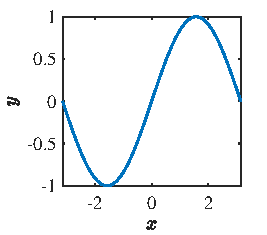
\includegraphics[width=5cm]{figures/chapter1/fig_demo.pdf}
  \bicaption{示意图}
  {Demo}
  \label{c1fig_demo1}
\end{figure}

图\ref{c1fig_demo2}是一行多列的子图安排方式。
\begin{figure}[!htb]
  \centering
  \subfigure[]{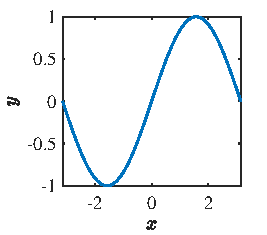
\includegraphics[width=0.28\textwidth]{figures/chapter1/fig_demo.pdf}}
  \subfigure[]{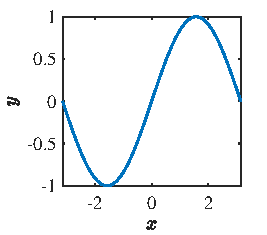
\includegraphics[width=0.28\textwidth]{figures/chapter1/fig_demo.pdf}}
  \bicaption{一行多列的子图安排方式。
  (a) 子图1,
  (b) 子图2}
  {Subfigure. 
  (a) subfigure 1,
  (b) subfigure 2} 
  \label{c1fig_demo2}
\end{figure}

图\ref{c1fig_demo3}是多行多列的子图安排方式。如果想让这段话出现在图\ref{c1fig_demo2}之后,则可以在图\ref{c1fig_demo2}中使用\verb|\begin{figure}[H]|命令。
\begin{figure}[H]
  \centering
  \subfigure[当然,如果你想,这里也可以写些内容]{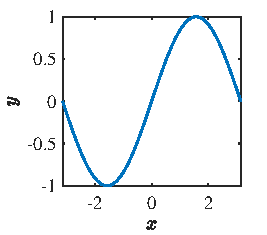
\includegraphics[width=0.28\textwidth]{figures/chapter1/fig_demo.pdf}}
  \subfigure[]{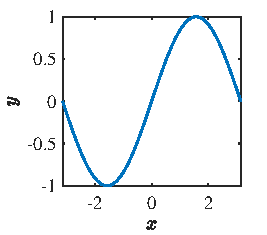
\includegraphics[width=0.28\textwidth]{figures/chapter1/fig_demo.pdf}}\\
  \subfigure[]{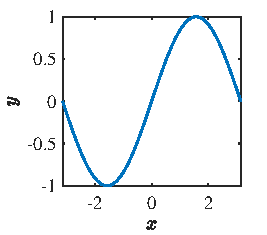
\includegraphics[width=0.28\textwidth]{figures/chapter1/fig_demo.pdf}}
  \subfigure[]{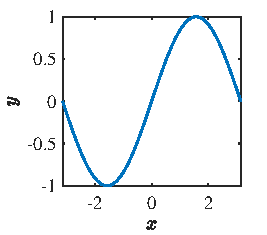
\includegraphics[width=0.28\textwidth]{figures/chapter1/fig_demo.pdf}}
  \bicaption{子图示意图。
  (a) 子图1,
  (b) 子图2,
  (c) 子图3,
  (d) 子图4}
  {Subfigure. 
  (a) subfigure 1,
  (b) subfigure 2,
  (c) subfigure 3,
  (d) subfigure 4} 
  \label{c1fig_demo3}
\end{figure}

% \newpage
\section{表格}\label{c1sec:table}

表\ref{c1tab_1}是一个标准的三线表格。
\begin{table}[H]
  \zihao{5} 
  \renewcommand{\arraystretch}{1.3}
  \renewcommand{\tabcolsep}{5pt}
  \bicaption{这是一个标准表格}
  {This is a standard table}
  \label{c1tab_1}
  \centering
  \begin{tabular}{cc}
  \toprule
  名称1 & 名称2 \\
  \midrule
  A	&	B	\\
  A	&	B	\\
  \bottomrule
  \end{tabular}
\end{table}

表\ref{c1tab_2}是一个带脚注的复杂表格。可以看到这段文字没有出现在上一页的末尾(尽管上一页的末尾还有空间),是因为表\ref{c1tab_1}中使用了\verb|\begin{table}[H]|命令。
\begin{table}[!htb]
  \zihao{5} 
  \renewcommand{\arraystretch}{1.3}
  \renewcommand{\tabcolsep}{5pt}
  \bicaption{这是一个带脚注的复杂表格\textsuperscript{a}}
  {This is a complex table}
  \label{c1tab_2}
  \centering
  \begin{tabular}{ccccccc}
  \toprule
  \multirow{3}{*}{AAA}	&	\multicolumn{2}{c}{BBB\textsuperscript{b}}	&	\multicolumn{2}{c}{CCC}	&	\multicolumn{2}{c}{DDD}	\\
  \cmidrule(r){2-3} \cmidrule(r){4-5} \cmidrule(r){6-7}
    &	\tabincell{c}{A1\\A2}	&	\tabincell{c}{B1\\B2}	&	\tabincell{c}{C1\\C2}	&	\tabincell{c}{D1\\D2}	&	\tabincell{c}{E1\\E2}	&	\tabincell{c}{F1\\F2}	\\
  \midrule
  AAA1	&	20361	&	27.02	&	20901	&	27.72	&	21711	&	28.14	\\
  AAA2	&	10051	&	13.34	&	10051	&	13.33	&	10311	&	13.36	\\
  \bottomrule
  \end{tabular}\\
  \textsuperscript{a} 脚注1 \\
  \textsuperscript{b} 脚注2 \\
\end{table}

表\ref{c1tab_3}是一个较宽的表格,需要缩放到页宽范围,这可以通过命令\\
\verb|\resizebox{1\textwidth}{!}{}|\\
实现。
此表格还采用了\verb|\specialrule{0pt}{3pt}{3pt}|命令来调整倒数第3行-倒数第2行的间距,使表格更美观。

\begin{table}[H]
  \zihao{5} 
  \bicaption{这是一个较宽的表格,需要缩放到页宽范围}
  {This is a complex table}
  \label{c1tab_3}
  \centering
  \resizebox{1\textwidth}{!}{ % 通过缩放,让宽表和正文一样宽
  \begin{tabular}{ccccccc}
  \toprule
  AAA	&	$\delta$	&	$\beta$\textsuperscript{\emph{a}}	&	\tabincell{c}{XXXXXXXXXXXX\\YYY}	&	\tabincell{c}{XXXXXXXXXXXX\\YYY}	&	\tabincell{c}{XXXXXXXXXXXX\\YYY}	&	\tabincell{c}{XXXXXXXXXXXX\\YYY}	\\
  \midrule
  \multirow{4}{*}{AAA}	&	2.549	&	2.549	&	30/30	&	30/30	&	30/30	&	30/30	\\
    &	AAA	&	2.718	&	30/30	&	30/30	&	30/30	&	30/30	\\
    &	AAA	&	3.094	&	30/30	&	30/30	&	30/30	&	30/30	\\
    &	AAA	&	3.200	&	30/30	&	30/30	&	30/30	&	30/30	\\ \specialrule{0pt}{3pt}{3pt}
  \multirow{2}{*}{BBB}	&	2.128	&	2.128	&	30/30	&	30/30	&	30/30	&	30/30	\\
    &	BBB	&	2.500	&	30/30	&	30/30	&	30/30	&	30/30	\\ 
  \bottomrule
  \end{tabular}}\\
  \textsuperscript{\emph{a}} 脚注1
\end{table}

当然,也可以将表\ref{c1tab_3}缩放到指定宽度,如80\%页面宽度,见表\ref{c1tab_4}。

\begin{table}[H]
  \zihao{5} 
  \bicaption{这是一个较宽的表格,需要缩放到80\%页宽范围}
  {This is a complex table}
  \label{c1tab_4}
  \centering
  \resizebox{0.8\textwidth}{!}{ % 通过缩放,让宽表和正文一样宽
  \begin{tabular}{ccccccc}
  \toprule
  AAA	&	$\delta$	&	$\beta$\textsuperscript{\emph{a}}	&	\tabincell{c}{XXXXXXXXXXXX\\YYY}	&	\tabincell{c}{XXXXXXXXXXXX\\YYY}	&	\tabincell{c}{XXXXXXXXXXXX\\YYY}	&	\tabincell{c}{XXXXXXXXXXXX\\YYY}	\\
  \midrule
  \multirow{4}{*}{AAA}	&	2.549	&	2.549	&	30/30	&	30/30	&	30/30	&	30/30	\\
    &	AAA	&	2.718	&	30/30	&	30/30	&	30/30	&	30/30	\\
    &	AAA	&	3.094	&	30/30	&	30/30	&	30/30	&	30/30	\\
    &	AAA	&	3.200	&	30/30	&	30/30	&	30/30	&	30/30	\\ \specialrule{0pt}{3pt}{3pt}
  \multirow{2}{*}{BBB}	&	2.128	&	2.128	&	30/30	&	30/30	&	30/30	&	30/30	\\
    &	BBB	&	2.500	&	30/30	&	30/30	&	30/30	&	30/30	\\ 
  \bottomrule
  \end{tabular}}\\
  \textsuperscript{\emph{a}} 脚注1
\end{table}


如果表格缩放到页面宽度后字体太小看不清,这时你可能需要通过使用\\
\verb|\begin{sidewaystable}|命令来实现一个横着放置的宽表,如表\ref{c1tab_5}所示。

\begin{sidewaystable}
  \zihao{5} 
  \renewcommand{\arraystretch}{1.2}
  % \renewcommand{\tabcolsep}{3pt}
  \bicaption{sidewaystable表格}
  {sidewaystable}
  \label{c1tab_5}
  \centering
  \begin{tabular}{ccc|cc|cc}
  \toprule
  Problem	&	AAA1	&	AAA2	&	BBB1	&	BBB2	&	CCC1	&	CCC2	\\
  \midrule
  ABC1	&	5.51e-01(8.20e-02)	&	\textbf{8.23e-01(1.75e-02)+ }	&	3.17e-02(3.99e-02)	&	\textbf{8.46e-01(9.72e-03)+ }	&	8.32e-01(9.47e-03)	&	\textbf{8.71e-01(1.51e-04)+ }	\\
  ABC2	&	2.38e-01(7.85e-02)	&	\textbf{4.81e-01(2.22e-02)+ }	&	0.00e+00(0.00e+00)	&	\textbf{9.77e-02(1.99e-01)+ }	&	4.48e-01(7.58e-02)	&	\textbf{5.38e-01(1.63e-04)+ }	\\
  ABC3	&	4.83e-01(6.85e-02)	&	\textbf{8.83e-01(9.03e-02)+ }	&	9.19e-02(6.93e-02)	&	\textbf{9.82e-01(3.03e-02)+ }	&	9.71e-01(1.49e-02)	&	\textbf{1.02e+00(3.01e-04)+ }	\\
  ABC4	&	0.00e+00(0.00e+00)	&	\textbf{5.83e-01(1.33e-01)+ }	&	0.00e+00(0.00e+00)	&	\textbf{9.58e-02(2.51e-01)+ }	&	1.55e-01(1.53e-01)	&	\textbf{6.77e-01(1.16e-01)+ }	\\
  ABC6	&	3.73e-01(7.27e-02)	&	\textbf{4.10e-01(2.62e-02)= }	&	1.39e-01(1.63e-01)	&	\textbf{1.79e-01(1.76e-01)= }	&	1.20e-01(7.40e-02)	&	\textbf{4.33e-01(1.39e-04)+ }	\\
  ABD1	&	1.21e+01(1.64e+00)	&	\textbf{4.31e+01(2.54e+00)+ }	&	1.58e+01(8.86e-01)	&	\textbf{4.49e+01(2.04e+00)+ }	&	2.74e+01(2.15e+00)	&	\textbf{3.34e+01(3.46e+00)+ }	\\
  ABD2	&	\textbf{5.54e+01(7.97e-01)}	&	5.51e+01(1.11e+00)= 	&	5.66e+01(5.68e-01)	&	\textbf{5.87e+01(3.75e-01)+ }	&	5.81e+01(4.11e-01)	&	\textbf{5.86e+01(3.19e-01)+ }	\\
  ABD4	&	2.86e+01(6.99e-01)	&	\textbf{3.27e+01(3.69e-01)+ }	&	3.06e+01(4.13e-01)	&	\textbf{3.40e+01(2.81e-01)+ }	&	3.38e+01(2.36e-01)	&	\textbf{3.49e+01(1.85e-01)+ }	\\
  ABD5	&	2.95e+01(3.10e-01)	&	\textbf{2.98e+01(4.45e-01)+ }	&	3.06e+01(2.38e-01)	&	\textbf{3.09e+01(2.48e-01)+ }	&	3.23e+01(2.38e-01)	&	\textbf{3.29e+01(1.74e-01)+ }	\\
  ABD6	&	2.47e+01(1.83e+00)	&	\textbf{2.83e+01(1.82e+00)+ }	&	2.67e+01(1.28e+00)	&	\textbf{2.98e+01(1.03e+00)+ }	&	3.08e+01(8.79e-01)	&	\textbf{3.12e+01(5.63e-01)= }	\\
  ABD7	&	2.87e+01(1.44e+00)	&	\textbf{3.25e+01(3.74e-01)+ }	&	3.22e+01(5.55e-01)	&	\textbf{3.41e+01(2.05e-01)+ }	&	3.40e+01(2.16e-01)	&	\textbf{3.44e+01(2.60e-01)+ }	\\
  ABD8	&	1.93e+01(2.52e+00)	&	\textbf{2.60e+01(8.95e-01)+ }	&	2.50e+01(6.55e-01)	&	\textbf{2.76e+01(2.78e-01)+ }	&	2.82e+01(3.08e-01)	&	\textbf{2.83e+01(3.76e-01)= }	\\
  ABD9	&	2.85e+01(1.72e+00)	&	\textbf{2.97e+01(1.87e+00)+ }	&	3.07e+01(1.21e+00)	&	\textbf{3.14e+01(1.74e+00)+ }	&	3.19e+01(7.18e-01)	&	\textbf{3.26e+01(3.73e-01)+ }	\\
  ABE1	&	4.93e-03(1.36e-02)	&	\textbf{1.09e-01(3.94e-02)+ }	&	2.70e-02(4.19e-02)	&	\textbf{1.09e-01(4.31e-02)+ }	&	5.89e-02(5.15e-02)	&	\textbf{8.66e-02(5.55e-02)+ }	\\
  ABE2	&	6.23e-01(2.53e-02)	&	\textbf{7.06e-01(1.98e-03)+ }	&	7.14e-01(2.33e-03)	&	\textbf{7.21e-01(2.34e-03)+ }	&	7.39e-01(8.54e-04)	&	\textbf{7.42e-01(4.94e-04)+ }	\\
  ABE3	&	0.00e+00(0.00e+00)	&	0.00e+00(0.00e+00)= 	&	\textbf{1.02e-03(5.60e-03)}	&	0.00e+00(0.00e+00)= 	&	0.00e+00(0.00e+00)	&	\textbf{1.18e-02(6.46e-02)= }	\\
  ABE4	&	5.26e-01(1.33e-01)	&	\textbf{5.34e-01(1.69e-01)= }	&	\textbf{4.76e-01(1.95e-01)}	&	4.57e-01(2.20e-01)= 	&	6.23e-01(1.66e-01)	&	\textbf{6.34e-01(1.42e-01)= }	\\
  ABE5	&	1.28e-01(6.25e-04)	&	\textbf{1.30e-01(1.27e-04)+ }	&	\textbf{1.26e-01(7.35e-04)}	&	1.25e-01(1.26e-03)- 	&	\textbf{1.29e-01(6.99e-04)}	&	1.28e-01(1.81e-03)= 	\\
  ABE6	&	1.09e-01(4.66e-02)	&	\textbf{1.29e-01(1.86e-03)+ }	&	1.17e-01(2.19e-02)	&	\textbf{1.18e-01(1.11e-02)+ }	&	\textbf{1.27e-01(1.04e-03)}	&	1.23e-01(1.14e-03)- 	\\
  ABE7	&	3.94e-01(2.29e-01)	&	\textbf{1.38e+00(3.38e-02)+ }	&	9.96e-02(1.76e-01)	&	\textbf{1.57e+00(3.60e-02)+ }	&	1.43e+00(5.21e-02)	&	\textbf{1.57e+00(1.15e-02)+ }	\\
  \midrule
  +/-/=	&		&	16/0/4	&		&	16/1/3	&		&	14/1/5	\\
  \bottomrule
  \end{tabular}
\end{sidewaystable}

\clearpage
如果一个表太长,则可能需要跨页表格,如表\ref{c1tab_long}所示。
\begin{center}
  \zihao{5} % 图、表、算法
  %\renewcommand{\arraystretch}{1.3} % longtable中的间距默认和正文一样
  \begin{longtable}{llrrr}
  \bicaption{这是一个长表}{This is a very long table}
  \label{c1tab_long} \\
  \toprule
  Name1	&	Name2	&	Name3	&	Name4	&	Name5	\\
  \midrule
  \endfirsthead
  \multicolumn{5}{r}{(接上表)}   \\
  \toprule
  Name1	&	Name2	&	Name3	&	Name4	&	Name5	\\
  \midrule
  \endhead
  AAA	&	A1	&	180.0	&	281.0	&	235.3	\\
      &	A2	&	5.3	&	43.5	&	35.1	\\
      &	A3	&	680.3	&	1020.0	&	759.3	\\
      &	A4	&	14.4	&	15.8	&	15.4	\\
      &	A5 	&	347.7	&	365.0	&	355.9	\\
      &	A6 	&	363.4	&	384.1	&	372.6	\\
      &	A7 	&	373.5	&	393.7	&	384.2	\\
      &	A8 	&	384.9	&	400.0	&	394.4	\\
      &	A9 	&	379.9	&	400.0	&	390.2	\\
      &	A10	&	379.5	&	399.7	&	390.2	\\
      &	A11	&	382.1	&	399.9	&	393.2	\\
  BBB	&	B1	&	895.8	&	918.8	&	907.2	\\
      &	B2	&	0.5	&	1.1	&	0.9	\\
      &	B3	&	715.6	&	2655.0	&	1360.1	\\
      &	B4	&	318.2	&	424.8	&	378.2	\\
      &	B5	&	183.0	&	242.0	&	215.0	\\
      &	B6	&	291.0	&	376.0	&	331.8	\\
      &	B7	&	373.0	&	452.0	&	429.6	\\
      &	B8	&	469.0	&	520.0	&	501.1	\\
      &	B9	&	521.0	&	565.0	&	549.5	\\
  CCC	&	C1&	912.7	&	947.5	&	929.2	\\
      &	C2	&	0.2	&	0.8	&	0.3	\\
      &	C3	&	143.0	&	229.0	&	184.7	\\
      &	C4	&	202.0	&	263.0	&	221.6	\\
      &	C5	&	243.0	&	304.0	&	269.9	\\
      &	C6	&	281.0	&	365.0	&	329.9	\\
      &	C7	&	293.0	&	379.0	&	342.3	\\
  DDD	&	D1	&	369.0	&	397.7	&	382.9	\\
      &	D2	&	384.6	&	406.7	&	394.6	\\
      &	D3	&	385.1	&	407.8	&	397.6	\\
      &	D4	&	388.3	&	405.1	&	398.7	\\
      &	D5	&	385.6	&	407.9	&	397.2	\\
      &	D6	&	387.4	&	414.5	&	401.6	\\
      &	D7	&	388.9	&	418.1	&	403.3	\\
      &	D8 	&	3.6	&	7.2	&	5.3	\\
      &	D9 	&	2.3	&	5.2	&	3.6	\\
      &	D10	&	11.8	&	23.9	&	17.6	\\
      &	D11	&	9.7	&	21.3	&	14.6	\\
      &	D12	&	34.4	&	42.6	&	39.2	\\
      &	D13	&	7.8	&	32.5	&	19.6	\\
  \bottomrule
  \end{longtable}
\end{center}%



\section{算法}\label{c1sec:algorithm}

下面是一个算法示例。

\begin{algorithm*}[!ht]
  \zihao{5} % 图、表、算法
\bicaption{算法示例}
{Algorithm demo}	
\label{c1alg_demo}
\begin{algorithmic}[1]
\Require{
$p_1$:参数1
\Statex	$p_1$:参数2
\Statex	$p_1$:参数3}
\Ensure{
$o_1$:输出1
\Statex	$o_2$:输出2}
\State    第一条命令   \Comment{第一条命令的注释}        
\While	{$True$}	
  \State /***** 下面代码块的注释 *****/
  \State 相关命令 \Comment{注释}
  \If  {$a=b$} \Comment{If的注释}
      \State 执行相关命令 \Comment{注释}
  \EndIf
  \If  {$c=d$}  
      \State 命令   \Comment{注释}
  \Else	
      \State  命令   \Comment{注释}
  \EndIf
\EndWhile
\Repeat
    \State   $j=j+1$ \Comment{注释}
\Until   {$j >  10$}
\For    {$i=1$ \textbf{to} $10$}
      \State $i=i+1$
\EndFor
\State \Return $o_1$, $o_2$
\end{algorithmic}
\end{algorithm*}


\section{公式}\label{c1sec:equation}

略。
更多公式排版见参考文献\cite{latexlive}。


\section{参考文献}\label{c1sec:reference}

参考文献样式分别上标(如参考文献\upcite{BITthesis,latexlive})和非上标(如参考文献\cite{BITthesis,latexlive},参考文献\cite{BITthesis}和\cite{latexlive})等样式。


\section{其他}\label{c1sec:other}

更多信息请参考文献\cite{BITthesis}。

关于LaTeX的更多知识参考文献\cite{LaTeX2e介绍}。

%% 参考文献内容(小4号宋体),使用 BibTeX,包含参考文献文件.bib
%\bibliography{reference/chap1,reference/chap2} %多个章节的参考文献
\bibliography{reference/references} %


%%%%%%%%%%%%%%%%%%%%%%%%%%%%%%
%% 后置部分
%%%%%%%%%%%%%%%%%%%%%%%%%%%%%%

%% 附录(章节编号重新计算,使用字母进行编号)
\appendix
\renewcommand\theequation{\Alph{chapter}--\arabic{equation}}  % 附录中编号形式是"A-1"的样子
\renewcommand\thefigure{\Alph{chapter}--\arabic{figure}}
\renewcommand\thetable{\Alph{chapter}--\arabic{table}}
% 附录
%\include{chapters/appendix1}

%(其后部分无编号)
\backmatter
% 致谢

\begin{thanks}

华东理工大学薛梦奇基于BIT-Thesis模板\upcite{BITthesis}做了一定修改,使其适用于华东理工大学的博士学位论文格式。
本文在其基础上进一步修改了部分内容(见第\ref{c1:intro}章第一段说明)。
对制作BIT-Thesis模板的各位老师、同学和薛梦奇师兄表示衷心的感谢。

\end{thanks}

% 发表文章目录
% 

\chapter*{攻读博士期间的主要学术成果及参与的科研项目}
\addcontentsline{toc}{chapter}{攻读博士期间的主要学术成果及参与的科研项目}


\noindent\textbf{学术论文:}
\begin{enumerate}
    \item 学术论文1
    \item 学术论文2
\end{enumerate}



\noindent\textbf{发明专利:}
\begin{enumerate}
    \item 发明专利1
\end{enumerate}


\noindent\textbf{软件著作:}
\begin{enumerate}
    \item 软件著作1
\end{enumerate}



\noindent\textbf{科研项目:}
\begin{enumerate}
    \item 项目1
    \item 项目2
\end{enumerate}






% \includepdf[pages=-]{chapters/卷内备考表.pdf}

\end{document}
